\documentclass[../../Rapport RayTracer.tex]{subfiles}


\begin{document}


Une autre exigence du sujet (en plus de l'ombrage de Phong section \ref{ombragePhong}) était également l'implémentation de réflexions. Nous avons donc implémenté la réflexion des matériaux à la façon des miroirs. Autrement dit, nous supposons que les matériaux réflechissants de notre ray tracer sont parfaitement lisses et renvoient les rayons de lumière dans une seule et unique direction. Nous avons pour cela utilisé un algorithme récursif. En effet, si notre rayon frappe, un objet réfléchissant, il sera renvoyé dans une autre direction. De nouveau, si ce nouveau rayon réfléchi rencontre un autre objet réfléchissant, il sera une fois de plus renvoyé et ainsi de suite. Un algorithme récursif s'applique alors très bien ici.

\begin{algorithm}[H]
	\DontPrintSemicolon
	\KwIn{$\overrightarrow{R}$ le rayon incident (partant de la caméra)\\
					 $depth$ la profondeur actuelle de récursion}
	\KwOut{La couleur du pixel du plan de l'image par lequel est passé le rayon\\\hfill\\}

	\If(\tcp*[h]{La profondeur de récursion maximale a été atteinte}){depth == 0}
	{
		\Return{Color.BLACK}
	}
	\hfill\\

	\If(\tcp*[h]{On vérifie si on a intersecté quelque chose}){$\overrightarrow{R}$.intersects(objetsScene)}
	{
		intersectedObject $\gets$ objet intersecté par $\overrightarrow{R}$\\\hfill\\

		\If(\tcp*[h]{Si l'objet intersecté est réfléchissant}){intersectedObject.isReflexive()}
		{
			$\overrightarrow{R_{reflect}} \gets$ computeReflectedDirection($\overrightarrow{R}$, $\overrightarrow{normale}$)\\\hfill\\

			\Return{computeReflection($\overrightarrow{R_{reflect}}$, depth - 1)}{\tcp*[h]{On effectue un appel récursif pour relancer un rayon dans la direction du rayon réfléchi}}
		}
		\Else(\tcp*[h]{L'objet n'est pas réfléchissant, on va simplement retourner son ombrage de Phong})
		{
			\Return{phongShading()}
		}
	}
	\Else(\tcp*[h]{On a rien intersecté})
	{
		\Return{backgroundColor}
	}

	\caption{Algorithme de calcul des réflexions pour des objets non colorés - computeReflection$(R, depth)$}
	\label{algoReflections}
\end{algorithm}
\hfill\\
L'algorithme lance un rayon et vérifie si une intersection avec un objet a été trouvée ou non. Si oui, on s'assure que l'objet est réfléchissant. Dans ce cas, nous calculons la direction du rayon réfléchi et faisons un appel récursif à computeReflection. Nous avons également défini une profondeur maximale de récursion (ou nombre de réflexion maximal) afin d'éviter les récursions infinies (un rayon coincé dans une boîte dont les faces seraient toutes réfléchissantes par exemple). Si l'objet n'est pas réfléchissant, nous renvoyons simplement son ombrage de Phong comme vu dans la section \ref{ombragePhong}. Une représentation graphique de ce principe de réflexion est donné en annexe \ref{annexe:reflexionsRecursives}.\\
Avec une scène contenant des sphères réfléchissantes, des sphères mattes et un plan pour le sol, nous obtenons le rendu suivant: 

\begin{figure}[h!]
	\adjustbox{center}{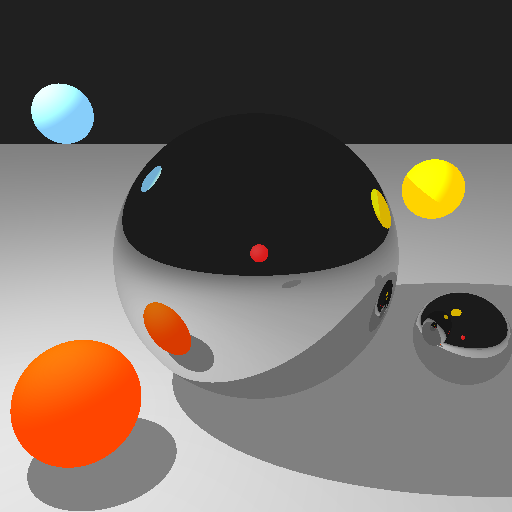
\includegraphics[width=0.5\textwidth]{img/rt/reflectionsDemo.png}}

	\caption{On peut voir une sphère rouge derrière la caméra grâce à la reflexion de la sphère centrale.}
	\label{reflectionsDemo}
\end{figure}
\FloatBarrier


\end{document}